\chapter{Change title for chapter 1 in chapters/01.tex}
Add content in chapters/01.tex.

\section{About literature}
\citet{Comrie1981} is a useful introduction to typology \is{typology}. %\is = index of subjects
It deals with languages of the whole world, not restricting itself to \ili{Indo-European languages}. %\il = index of languages
\iai{Dionysios Thrax} was also an important figure. %\ia = index of authors. Not necessary for authors whose work you cite.

Lorem\footnote{This is a footnote} ipsum dolor sit 
amet,\footnote{This is a footnote consectetur adipiscing elit. In luctus pharetra dui, imperdiet vulputate risus pretium non.} Aliquam eget efficitur eros, vel efficitur lectus. Sed a enim libero. Ut posuere velit lectus, vel porta quam posuere vel. Cras in dolor tincidunt erat malesuada malesuada. Quisque elementum nibh id nisl pretium, et rutrum est pellentesque. Curabitur efficitur condimentum tempor. Vivamus venenatis, libero quis blandit volutpat, risus massa ullamcorper neque, et condimentum quam orci sed dui. Ut iaculis tempor enim quis rhoncus. Maecenas imperdiet ultricies nunc, eu sagittis nulla maximus a. Etiam imperdiet eleifend ante. Sed felis sem, sollicitudin vitae ultrices eget, sagittis nec nulla. Donec eget libero maximus, fermentum nibh et, maximus libero. Sed auctor est vel lacus lobortis sollicitudin. Maecenas dapibus nisi leo, sed elementum nisl aliquet ac. Aliquam lobortis, ante in accumsan dignissim, enim odio mattis ex, quis molestie risus lectus et risus. 

\ea\label{ex:1:descartes}
\langinfo{Latin}{}{personal knowledge}\\
\gll cogit-o ergo sum \\
     think-1{\SG}.{\PRS}.{\IND} hence exist.1{\SG}.{\PRS}.{\IND}\\
\glt `I think therefore I am'
\z

Duis eu interdum urna. In et enim in nibh tincidunt pellentesque. In vestibulum nibh at convallis auctor. Proin porta nisi auctor turpis tristique, eu gravida dolor ultricies. Vivamus pellentesque, erat vel dignissim ornare, neque metus gravida libero, at posuere est ipsum tincidunt metus. Cras a ornare mi, a venenatis justo. Quisque arcu lacus, consectetur in sollicitudin congue, tincidunt at quam. Aliquam tempus tortor nec diam pulvinar porttitor. Nulla scelerisque leo vel orci venenatis, congue consequat urna mattis. Donec dui velit, luctus vitae placerat vitae, tincidunt vitae quam. Vivamus est est, fringilla et est sed, rutrum ornare lectus. Aenean non urna eu urna pharetra porta. Praesent mollis justo ipsum. 

\begin{table}
\caption{Frequencies of word classes}
\label{tab:1:frequencies}
 \begin{tabular}{lllll} % add l for every additional column or remove as necessary
  \lsptoprule
            & nouns & verbs & adjectives & adverbs\\ %table header
  \midrule
  absolute  &   12 &    34  &    23     & 13\\
  relative  &   3.1 &   8.9 &    5.7    & 3.2\\
  \lspbottomrule
 \end{tabular}
\end{table}


Sed vitae lorem lectus. Nunc sit amet venenatis risus. Nullam a metus vitae ligula porttitor mollis. Aenean sit amet faucibus ligula, vitae molestie leo. Suspendisse at ligula ante. Sed posuere mauris et iaculis imperdiet. Suspendisse potenti. Donec in nisi id elit ultricies sollicitudin ac eget augue. Nulla pellentesque, libero ac faucibus suscipit, odio neque tempus elit, nec dictum dolor enim sit amet leo. 

\begin{figure}
\caption{Some XML}
\begin{lstlisting}
<LogEvent Action = "1" Value = "107" Cursor = "477">
<LogEvent Action = "1" Value = "107" Cursor = "477">
<LogEvent Action = "1" Value = "107" Cursor = "477">
<LogEvent Action = "1" Value = "107" Cursor = "477">
\end{lstlisting}
\end{figure}

%\begin{figure} 
%  \langscidata{data/dataset1.csv}
%  \begin{tikzpicture}
%    \begin{langscibars}
%	\langscibar{English}
%	\langscibar{Spanish}
%	\langscibar{French}
%	\langscibar{Italian} 
%    \end{langscibars} 
%  \end{tikzpicture}
%  \caption{Barplot from dataset}
%\end{figure}

\begin{figure}
  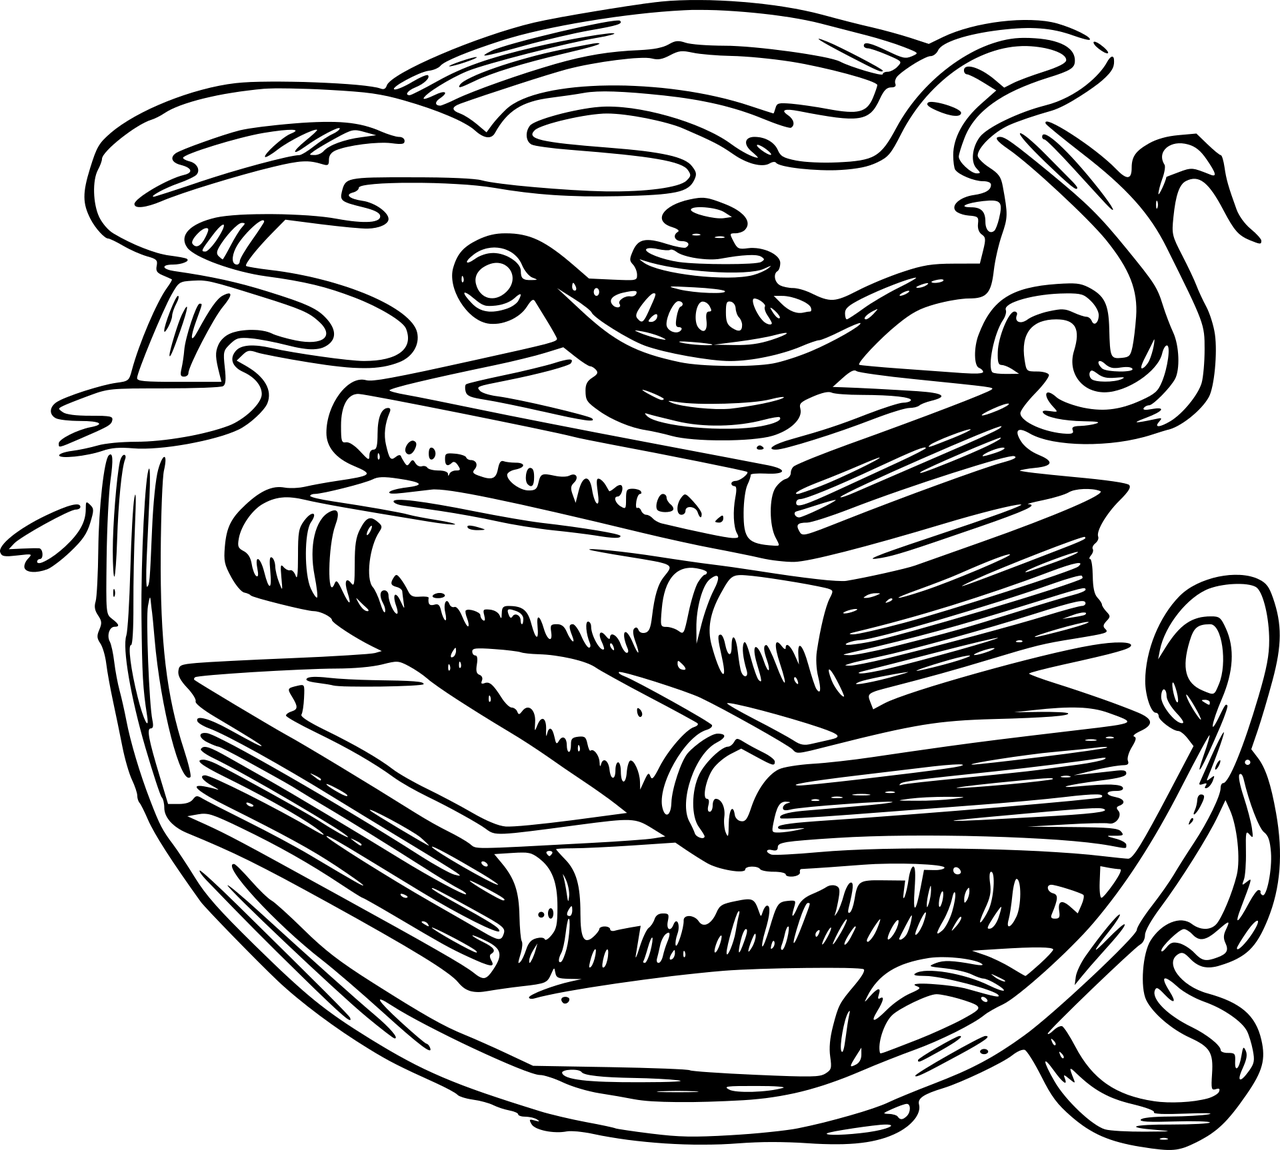
\includegraphics[width=\textwidth]{figures/samplefigure.png}
  \caption{\label{fig:samplefigure}A sample figure}
\end{figure}

 
\citet{Nordhoff2018} is useful for compiling bibliographies.
